\section{Cohort, rules and outcomes}
\label{app:cohort}

\begin{longtable}{rrrrrlr}
\caption{The twenty-game cohort. Seats and rotations are one-based. Games 1--4 and 5--20 carry different treatment fingerprints.}\label{tab:cohort}\\
\toprule Game & Block & Seed & Rotation & Turns & Winner & Winner seat\\\midrule\endfirsthead
\toprule Game & Block & Seed & Rotation & Turns & Winner & Winner seat\\\midrule\endhead
1 & 1 & 751774554 & 1 & 216 & Gemini & 3\\
2 & 1 & 751774554 & 2 & 102 & Gemini & 2\\
3 & 1 & 751774554 & 3 & 283 & Gemini & 1\\
4 & 1 & 751774554 & 4 & 166 & Grok & 1\\
5 & 2 & 2506298840 & 1 & 170 & Sol & 2\\
6 & 2 & 2506298840 & 2 & 126 & Sol & 1\\
7 & 2 & 2506298840 & 3 & 150 & Sol & 4\\
8 & 2 & 2506298840 & 4 & 139 & Sol & 3\\
9 & 3 & 2573692901 & 1 & 88 & Sol & 2\\
10 & 3 & 2573692901 & 2 & 75 & Gemini & 2\\
11 & 3 & 2573692901 & 3 & 145 & Grok & 2\\
12 & 3 & 2573692901 & 4 & 166 & Opus & 2\\
13 & 4 & 3648314310 & 1 & 185 & Opus & 1\\
14 & 4 & 3648314310 & 2 & 110 & Sol & 1\\
15 & 4 & 3648314310 & 3 & 114 & Gemini & 1\\
16 & 4 & 3648314310 & 4 & 386 & Sol & 3\\
17 & 5 & 2766649504 & 1 & 118 & Sol & 2\\
18 & 5 & 2766649504 & 2 & 197 & Opus & 4\\
19 & 5 & 2766649504 & 3 & 175 & Gemini & 1\\
20 & 5 & 2766649504 & 4 & 115 & Gemini & 4\\
\bottomrule\end{longtable}


\begin{figure}[htbp]
\centering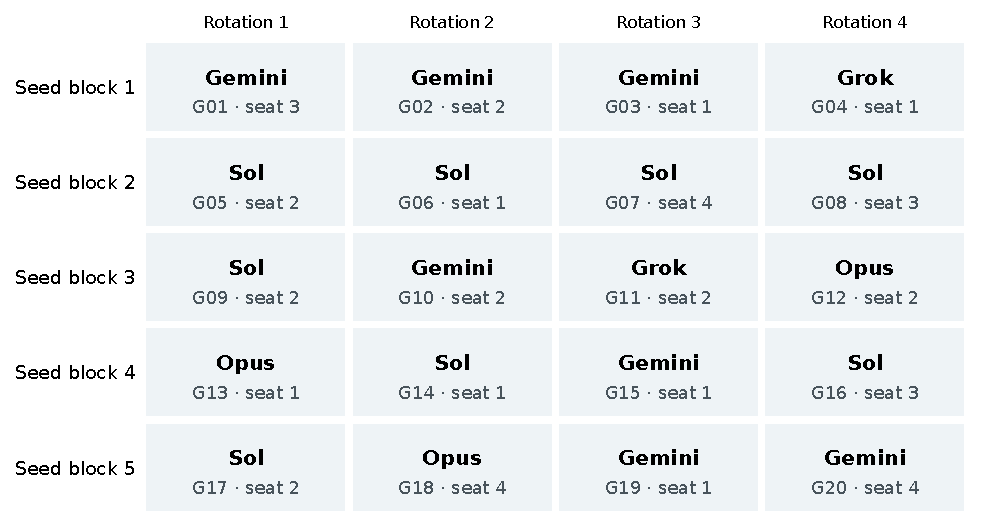
\includegraphics[width=0.9\linewidth]{cohort.pdf}
\caption{Winner and winning seat in all twenty games. Each row shares a seed and contains four cyclic rotations. Sol wins every game in block 2; seat 2 wins every game in block 3 under four different configurations. These are descriptive outcomes, not independent trials of a ranking. The figure is placed here, rather than first in the paper, so that it is not read as a leaderboard.}
\label{fig:cohort}
\end{figure}

The saved ruleset is \texttt{audit\_corrected\_v2}. Beyond Section~\ref{sec:rules}: Free Parking pays nothing; income and luxury taxes are \$200 and \$100; a player in jail may try three times for doubles before a forced fine; and the public state names each opponent's configured model. Trade transfer interest computes ten percent of the mortgage value and equals the exact charge for every principal on this board. Redemption computes 1.1 times the principal with a floating-point ceiling, which exceeds the exact charge by one dollar for principals of \$50, \$90, \$100, \$110 and \$200. A model expecting \$110 for a \$100 mortgage is therefore right about the standard rule and wrong about this engine. The construction validator checks even building after every build-plan entry, while the sale validator checks final evenness and net stock, so a bundled sale can be legal although no atomic ordering of its parts is offered on the menu. A player who remains in jail receives no management window that turn.

Two treatment fingerprints separate games 1--4 from games 5--20 (source commits \texttt{42f85183} and \texttt{d6808534}). An earlier inspection of their eighteen-file diff found campaign-concurrency, application, documentation and test changes, but no engine, prompt, decision-resolver, player-configuration or OpenRouter-client change. That inspection does not identify or rule out an effect of the change.
